% This must be in the first 5 lines to tell arXiv to use pdfLaTeX, which is strongly recommended.
\pdfoutput=1
% In particular, the hyperref package requires pdfLaTeX in order to break URLs across lines.

\documentclass[11pt]{article}

% Remove the "guidelines" option to generate the final version.
%\usepackage[guidelines]{nlpreport} % show guidelines
\usepackage[]{nlpreport} % hide guidelines


% Standard package includes
\usepackage{times}
\usepackage{latexsym}

% For proper rendering and hyphenation of words containing Latin characters (including in bib files)
\usepackage[T1]{fontenc}
% For Vietnamese characters
% \usepackage[T5]{fontenc}
% See https://www.latex-project.org/help/documentation/encguide.pdf for other character sets

% This assumes your files are encoded as UTF8
\usepackage[utf8]{inputenc}

% This is not strictly necessary, and may be commented out,
% but it will improve the layout of the manuscript,
% and will typically save some space.
\usepackage{microtype}
\usepackage{graphicx}
\usepackage{hyperref}
\usepackage{amsmath}
\usepackage{mathtools}
\usepackage{multirow}
\usepackage{listings}
\usepackage{xcolor}
\usepackage{booktabs} % for tables
\usepackage{float}






% THE pdfinfo Title AND Author ARE NOT NECESSARY, THEY ARE METADATA FOR THE FINAL PDF FILE
\hypersetup{pdfinfo={
Title={Question Answering (QA) on CoQA dataset: a conversational QA dataset.},
Author={Vincenzo Collura, Gianmarco Pappacoda, Anthea Silvia Sasdelli\\}
}}

%\setcounter{secnumdepth}{0}  
 \begin{document}
%
\title{Assignment 2\\
Question Answering (QA) on CoQA dataset: a conversational QA dataset.
}
\author{Vincenzo Collura,
Gianmarco Pappacoda,
\and
Anthea Silvia Sasdelli\\
Master's Degree in Artificial Intelligence, University of Bologna\\
\{ vincenzo.collura2, gianmarco.pappacoda, anthea.sasdelli \}@studio.unibo.it
}
\maketitle


\attention{DO NOT MODIFY THIS TEMPLATE - EXCEPT, OF COURSE FOR TITLE, SUBTITLE AND AUTHORS.\\ IN THE FINAL VERSION, IN THE \LaTeX\ SOURCE REMOVE THE \texttt{guidelines} OPTION FROM  \texttt{$\backslash$usepackage[guidelines]\{nlpreport\}}.
}

\begin{abstract}
%\begin{quote}

\explanation{
The abstract is very brief summary of your report. Try to keep it no longer than 15-20 lines at most. Write your objective, your approach, and your main observations (what are the findings that make this report worthwhile reading?)}

Question Answering (QA) is a relevant task of Natural Language Processing, albeit simple it comes in many different forms and evaluating text comprehension is a matter of debate. The objective of this report is to explore the use of two Large Language Models (LLM) used in an encoder-decoder fashion to perform QA on the CoQA. The task is considered in two variants: with and without considering dialogue history.


%\end{quote}
\end{abstract}

\attention{\textcolor{red}{NOTICE: THIS REPORT'S LENGTH MUST RESPECT THE FOLLOWING PAGE LIMITS: \begin{itemize}
    \item ASSIGNMENT: \textbf{2 PAGES} 
    \item NLP PROJECT OR PROJECT WORK: \textbf{8 PAGES}
    \item COMBINED NLP PROJECT + PW: \textbf{12 PAGES}
\end{itemize}  PLUS LINKS, REFERENCES AND APPENDICES.\\ 
THIS MEANS THAT YOU CANNOT FILL ALL SECTIONS TO MAXIMUM LENGTH. IT ALSO MEANS THAT, QUITE POSSIBLY, YOU WILL HAVE TO LEAVE OUT OF THE REPORT PART OF THE WORK YOU HAVE DONE OR OBSERVATIONS YOU HAVE. THIS IS NORMAL: THE REPORT SHOULD EMPHASIZE WHAT IS MOST SIGNIFICANT, NOTEWORTHY, AND REFER TO THE NOTEBOOK FOR ANYTHING ELSE.\\ 
FOR ANY OTHER ASPECT OF YOUR WORK THAT YOU WOULD LIKE TO EMPHASIZE BUT CANNOT EXPLAIN HERE FOR LACK OF SPACE, FEEL FREE TO ADD COMMENTS IN THE NOTEBOOK.\\ 
INTERESTING TEXT EXAMPLES THAT EXCEED THE MAXIMUM LENGTH OF THE REPORT CAN BE PLACED IN A DEDICATED APPENDIX AFTER THE REFERENCES.}}


\section{Introduction}
\label{sec:introduction}
\attention{MAX 1 COLUMN FOR ASSIGNMENT REPORTS / 2 COLUMNS FOR PROJECT OR PW / 3 FOR COMBINED REPORTS.}
Question Answering systems are becoming increasingly necessary as many tasks can benefit from a prompt reply to a given question.
Most Question Answering systems work in the following way: given a passage (often called context) and a question, they try to extract a span of text that answers the question.
In the given task, the models should generate an answer rather than extracting it from the context. Two variants of the task have been considered:
\begin{itemize}
\item \textbf{Question+Context:} as described above.
\item \textbf{Question+Context+History:} the question/context pair is enriched with previous passages in the dialogue.
\end{itemize}

The dataset given for this assignment is the Conversational Question Answering Challenge (CoQA) \cite{Reddy2018}. As in the dataset a number of unanswerable QA pairs is present ($1.3\%$), they have been removed as per instructions.

In order to evaluate the impact of the history, two models have been created:
\begin{itemize}
\item $A = f_\theta(Q,P)$
\item $A = f_\theta(Q,P,H)$
\end{itemize}
Where $Q$ is the question, $P$ is the text passage (context), $H$ is the dialogue history, $A$ is the generated answer and $f_\theta$ is the transformer-based model with $\theta$ parameters.

%All this was done in seven subtasks:
%the first one is the removal of the unaswerable QA pairs, done after the download and the inspection of the data.
%The second task is the dataset splitting in test, validation and train.
%The third task is the definition of the two neural models.
%The following two steps are respectively the question generation with text passage and question, with and without consider %the dialogue history.
%Then the models are trained and evaluated in the sixth step and the errors are analyzed in the seventh step.


\explanation{
The Introduction is an executive summary, which you can think of as an extended abstract.  Start by writing a brief description of the problem you are tackling and why it is important. (Skip it if this is an assignment report).} 

\explanation{Then give a short overview of known/standard/possible approaches to that problems, if any, and what are their advantages/limitations.} 

\explanation{After that, discuss your approach, and motivate why you follow that approach. If you are drawing inspiration from an existing model, study, paper, textbook example, challenge, \dots, be sure to add all the necessary references~\cite{DBLP:journals/corr/abs-2204-02311,DBLP:conf/acl/LorenzoMN22,DBLP:conf/clef/AnticiBIIGR21,DBLP:conf/ijcai/NakovCHAEBPSM21,DBLP:conf/naacl/RottgerVHP22,DBLP:journals/toit/LippiT16}.\footnote{\href{https://en.wikipedia.org/wiki/The_Muppet_Show}{Add only what is relevant.}}}

\explanation{Next, give a brief summary of your experimental setup: how many experiments did you run on which dataset. Last, make a list of the main results or take-home lessons from your work.}

\attention{HERE AND EVERYWHERE ELSE: ALWAYS KEEP IN MIND THAT, CRUCIALLY, WHATEVER TEXT/CODE/FIGURES/IDEAS/... YOU TAKE FROM ELSEWHERE MUST BE CLEARLY IDENTIFIED AND PROPERLY REFERENCED IN THE REPORT.}


\section{System description}
\label{sec:system}
\attention{MAX 1 COLUMN FOR ASSIGNMENT REPORTS / 4 COLUMNS FOR PROJECT OR PW / 6 FOR COMBINED REPORTS.}

The system can be synthesized as follows:
\begin{itemize}
\item Preprocessing
\item Model instantiation
\item Tokenization
\item Training
\item Answer generation (Inference)
\end{itemize}

The above steps have been implemented through a wrapper which abstracts the main function expected of these models from the underlying interface (HuggingFace transformers/datasets libraries).

The data preprocessing has been kept to a minimum as per instructions, the only preprocessing step being the removal of unanswerable QA pairs. As for history, each previous QA pair is encoded as text and is appended to the context.

The proposed models have been implemented using an Encoder-Decoder architecture, where Large Language Models (LLMs) are used to encode a given input and produce a given output. In the task at hand, this architecture is leveraged to repurpose LLMs for task they have not been trained for, a form of transfer learning.

The tokenizer, the component responsible for tokenization, is wrapped alongside the underlying model as it is dependent on it.

The training step is once again a wrap of Hugging Face Seq2SeqTrainer.

The inference step can be performed in many different ways as the answer is generated rather than extracted. Three main methods have been implemented: \textbf{Beam Search}, \textbf{Top-K} and \textbf{Greedy Search}.

As LLMs impose a hard constraint on resources needed for training, the following two ``distilled'' versions of popular LLMs have been employed:

\begin{itemize}
\item \texttt{BERT-Tiny} \cite{Bhargava2021, Turc2019}
This is one of the smaller pre-trained BERT variants..
\item \texttt{DistilRoBERTa-base} \cite{Sanh2019}
\end{itemize}

As even the two ``distilled'' versions of the proposed LLMs proved to be heavy for the authors' resources, the weights of the encoder and decoder parts have been tied as it has been empirically proven to only slightly reduce performance \cite{Rothe2020}.

\explanation{
Describe the system or systems you have implemented (architectures, pipelines, etc), and used to run your experiments. If you reuse parts of code written by others, be sure to make very clear your original contribution in terms of
\begin{itemize}
    \item architecture: is the architecture your design or did you take it from somewhere else
    \item coding: which parts of code are original or heavily adapted? adapted from existing sources? taken from external sources with minimal adaptations?
\end{itemize}
It is a good idea to add figures to illustrate your pipeline and/or architecture(s)
(see Figure~\ref{fig:architecture})
%
\begin{figure*}
    \centering
    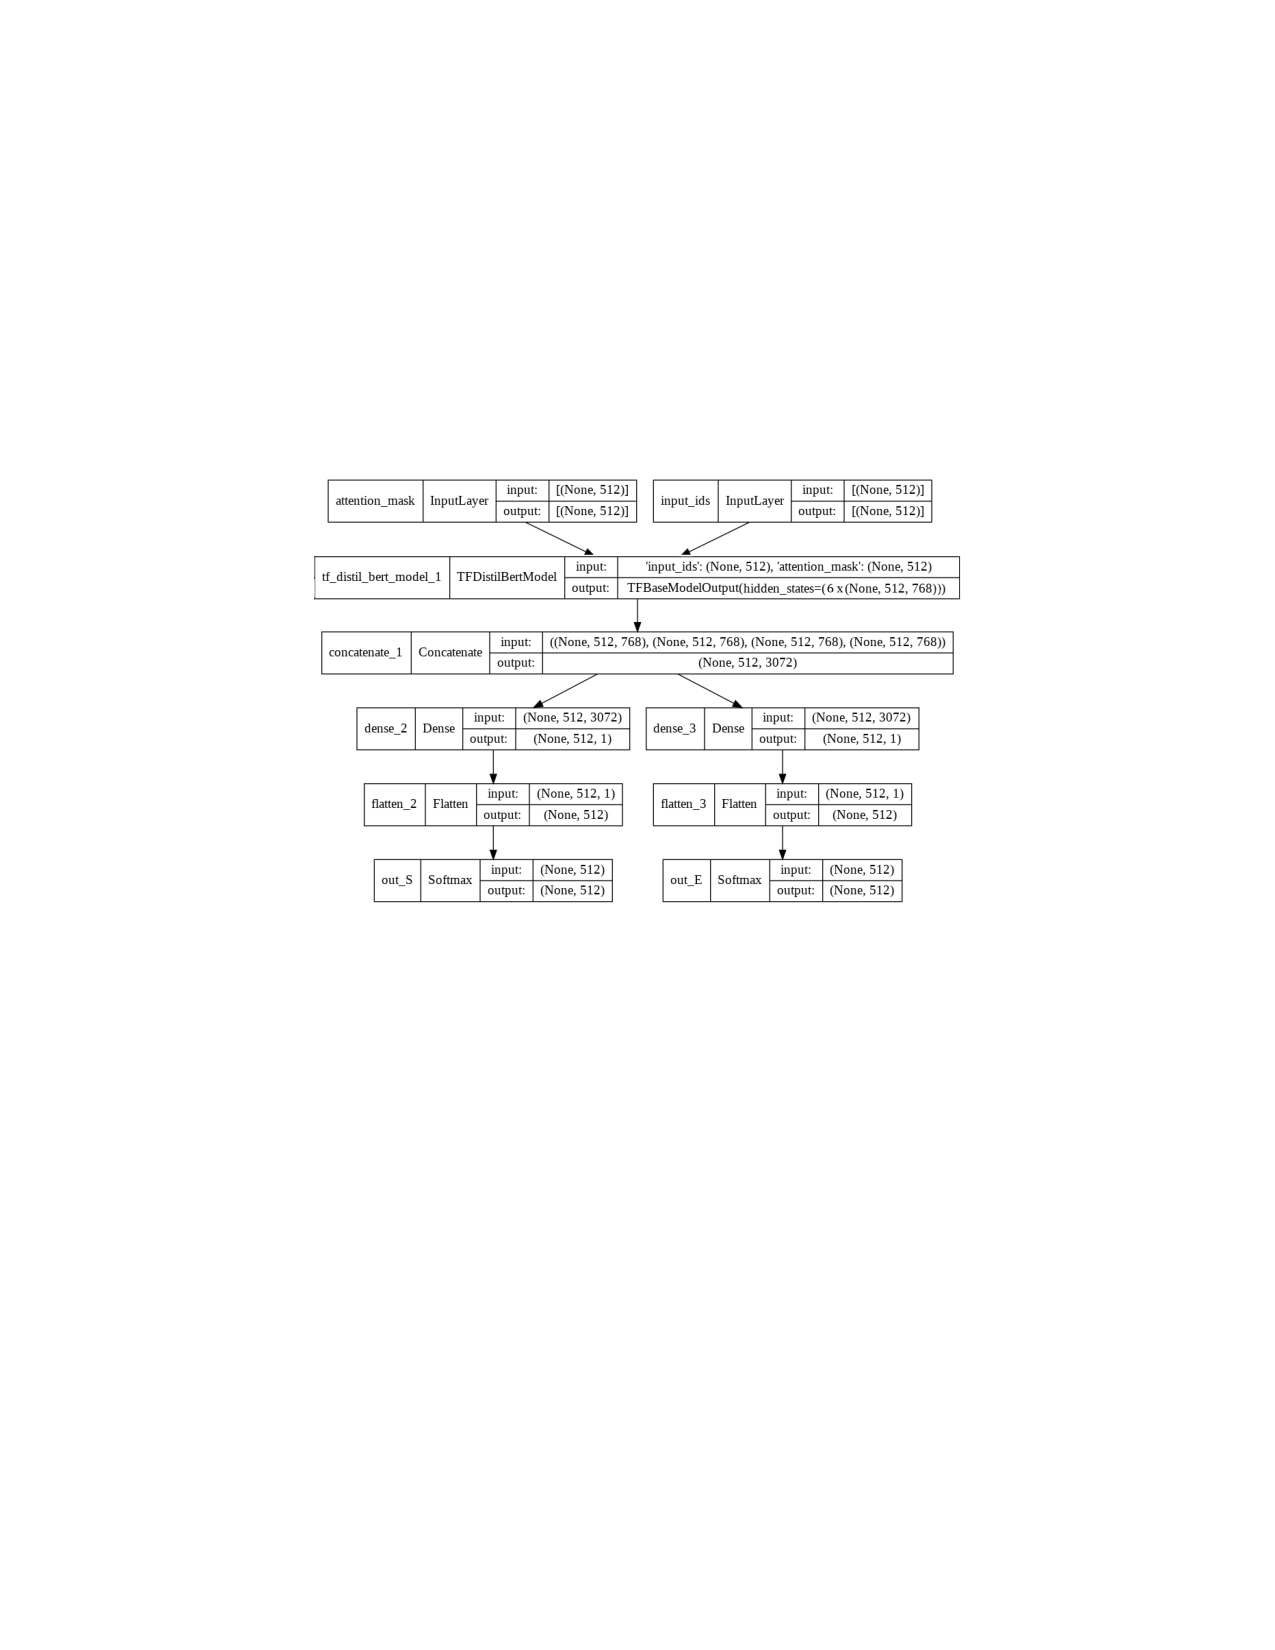
\includegraphics[width=\textwidth]{img/architecture.pdf}
    \caption{Model architecture}
    \label{fig:architecture}
\end{figure*}
}

% \section{Data}
% \label{sec:data}
% \attention{MAX 2 COLUMNS / 3 FOR COMBINED REPORTS. OMIT SECTION IN ASSIGNMENT REPORTS.}

% The dataset used in this assignment is the CoQA, a large-scale dataset for building Conversational Question Answering systems. It consists of 127k conversation turns collected from 8k conversations over text passages in 7 diverse domains. The average conversation length is 15 turns, and each turn consists of a question and an answer. Only train and validation sets are available for this dataset, reason why the train has been split in train and validation splits (80\% train and 20\% val), performing that split such that a dialogue appears in one split only. In order to have more general and inclusive functions also the history column is added to the dataframes. After the processing and the splitting of the data, some columns are dropped, leaving a cleaner dataframe with just source, context, question, answer and history columns.


% \explanation{Provide a brief description of your data including some statistics and pointers (references to articles/URLs) to be used to obtain the data. Describe any pre-processing work you did. Links to datasets must be placed later in Section~\ref{sec:links}.}

\section{Experimental setup and results}
\label{sec:results}
\attention{MAX 1 COLUMN FOR ASSIGNMENT REPORTS / 3 COLUMNS FOR PROJECT OR PW / 5 FOR COMBINED REPORTS.}

The data was split into training and validation sets, with a $80\%$ ratio. The test set is already provided.
During each experiment the Random Number Generator (RNG) of all the involved frameworks has been fixed to ensure reproducibility. The experiments, both training and evaluation, are repeated using three different seeds. 

The most important hyperparameters available for tweaking are: learning rate, batch size and text generation method. Bert-tiny models have been trained using $lr=10^{-3}$, distilroberta-base ones with $lr=2\cdot10^{-5}$.

During the evaluation step, the models are evaluated against the validation and test set performing text generation using \textbf{Beam search}. The text generation method is tweak-able, Beam search has been observed to empirically produce the best results.

The metric selected for evaluation is the SQUAD F1-score\cite{Rajpurkar2018} (implementation thanks to \cite{Gardner2017}). 


\begin{table}[H]
\centering
\resizebox{\columnwidth}{!}{%
\begin{tabular}{@{}lcrlll@{}}
\toprule
        &      & \multicolumn{2}{c}{Bert-Tiny} & \multicolumn{2}{l}{DistilRoBERTa-base} \\ \midrule
History & seed & \multicolumn{4}{c}{squad f1-score}                                     \\
        &      & val           & test          & val                & test              \\ \midrule
        & 42   & 0.1639        & 0.1638        & 0.1728             & 0.1770            \\
No      & 2022 & \textbf{0.1705}        & \textbf{0.1700}        & 0.1752             & 0.1712            \\
        & 1337 & 0.1701        & 0.1645        & \textbf{0.1870}             & \textbf{0.1873}            \\ \midrule
        & 42   & 0.1700        & \textbf{0.1710}        & 0.1732             & 0.1759            \\
Yes     & 2022 & 0.1702        & 0.1699        & 0.1780             & 0.1704            \\
        & 1337 & \textbf{0.1738}        & 0.1646        & \textbf{0.2074}             & \textbf{0.2033}            \\ \bottomrule
\end{tabular}%
}
\end{table}

\explanation{
Describe how you set up your experiments: which architectures/configurations you used, which hyper-parameters and what methods used to set them, which optimizers, metrics, etc.
\\
Then, \textbf{use tables} to summarize your your findings (numerical results) in validation and test. If you don't have experience with tables in \LaTeX, you might want to use \href{https://www.tablesgenerator.com/}{\LaTeX table generator} to quickly create a table template.
}


\section{Discussion}
\label{sec:discussion}
\attention{MAX 1.5 COLUMNS FOR ASSIGNMENT REPORTS / 3 COLUMNS FOR PROJECT / 4 FOR COMBINED REPORTS. ADDITIONAL EXAMPLES COULD BE PLACED IN AN APPENDIX AFTER THE REFERENCES IF THEY DO NOT FIT HERE.}


\explanation{
Here you should make your analysis of the results you obtained in your experiments. Your discussion should be structured in two parts: 
\begin{itemize}
    \item discussion of quantitative results (based on the metrics you have identified earlier; compare with baselines);
    \item error analysis: show some examples of odd/wrong/unwanted  outputs; reason about why you are getting those results, elaborate on what could/should be changed in future developments of this work.
\end{itemize}
}

While it has been possible to implement the system and the experiments, the resulting models have been unable to provide satisfactory results. Most of the answers generated by the models are wrong, albeit they show a striking resemblance with an answer that makes sense: the models produce answers that are in the domain of the correct answer.

The addendum of the history has not yielded significantly better models results compared to the baseline versions that did not feature history as an input. This is partly due to the fact the history is appended to the context, the models maximum input length limits its effectiveness.

The obtained results are lacking with respect to the selected metric but show interesting patterns in the learning process of the models. As most answers are considered wrong, it is not possible to assess common errors. It is, instead, feasible to observe that most correct answers are closed-form yes/no answers.

\section{Conclusion}
\label{sec:conclusion}
\attention{MAX 1 COLUMN.}

\explanation{
In one or two paragraphs, recap your work and main results.
What did you observe? 
Did all go according to expectations? 
Was there anything surprising or worthwhile mentioning?
After that, discuss the main limitations of the solution you have implemented, and indicate promising directions for future improvement.
}

It has been possible to implement all the given tasks. The models employing history have been empirically proven to be slightly superior with respect to their non-history variants. While it has been possible to obtain some results, the limit on the number of epochs and the lack of required equipment to train the models have severely limited the possibility to obtain significative results. As a result of this the error analysis did not highlight anything in particular as both models are incapable of answering to most questions and most of the positive results are due to closed yes/no questions.

Moreover, the method used to implement history (i.e. concatenating history and context) has proven to be somewhat useful, but it is once again limited by the input length which is in turn limited by the available resources to train the model. A different approach would have required different architectures and/or multiple networks, which was again, not allowed.

Overall distilroberta-base performed only slightly better compared to bert-tiny (w.r.t squad-f1) while using many more parameters, resources.

% \section{Links to external resources}
% \label{sec:links}
% \attention{THIS SECTION IS OPTIONAL}
% \explanation{
% Insert here:
% \begin{itemize}
%    \item a link to your GitHub or any other public repo where one can find your code (only if you did not submit your code on Virtuale); 
%    \item a link to your dataset (only for non-standard projects or project works).
% \end{itemize}
% }

\attention{DO NOT INSERT CODE IN THIS REPORT}




\bibliography{nlpreport.bib}
\end{document}